% Thank you Josh Davis for this template!
% https://github.com/jdavis/latex-homework-template/blob/master/homework.tex

\documentclass{article}

\newcommand{\hmwkTitle}{HW\ \#3}

% % ----------

% Packages

\usepackage{fancyhdr}
\usepackage{extramarks}
\usepackage{amsmath}
\usepackage{amssymb}
\usepackage{amsthm}
\usepackage{amsfonts}
\usepackage{tikz}
\usepackage[plain]{algorithm}
\usepackage{algpseudocode}
\usepackage{enumitem}
\usepackage{chngcntr}

% Libraries

\usetikzlibrary{automata, positioning, arrows}

%
% Basic Document Settings
%

\topmargin=-0.45in
\evensidemargin=0in
\oddsidemargin=0in
\textwidth=6.5in
\textheight=9.0in
\headsep=0.25in

\linespread{1.1}

\pagestyle{fancy}
\lhead{\hmwkAuthorName}
\chead{}
\rhead{\hmwkClass\ (\hmwkClassInstructor): \hmwkTitle}
\lfoot{\lastxmark}
\cfoot{\thepage}

\renewcommand\headrulewidth{0.4pt}
\renewcommand\footrulewidth{0.4pt}

\setlength\parindent{0pt}
\setcounter{secnumdepth}{0}

\newcommand{\hmwkClass}{MATH 3380 / Analysis 1}        % Class
\newcommand{\hmwkClassInstructor}{Dr. Welsh}           % Instructor
\newcommand{\hmwkAuthorName}{\textbf{Joshua Mitchell}} % Author

%
% Title Page
%

\title{
    \vspace{2in}
    \textmd{\textbf{\hmwkClass:\ \hmwkTitle}}\\
    \normalsize\vspace{0.1in}\small\vspace{0.1in}\large{\textit{\hmwkClassInstructor}}
    \vspace{3in}
}

\author{\hmwkAuthorName}
\date{}

\renewcommand{\part}[1]{\textbf{\large Part \Alph{partCounter}}\stepcounter{partCounter}\\}

% Integral dx
\newcommand{\dx}{\mathrm{d}x}

%
% Various Helper Commands
%

% For derivatives
\newcommand{\deriv}[1]{\frac{\mathrm{d}}{\mathrm{d}x} (#1)}

% For partial derivatives
\newcommand{\pderiv}[2]{\frac{\partial}{\partial #1} (#2)}


% Alias for the Solution section header
\newcommand{\solution}{\textbf{\large Solution}}

% Probability commands: Expectation, Variance, Covariance, Bias
\newcommand{\E}{\mathrm{E}}
\newcommand{\Var}{\mathrm{Var}}
\newcommand{\Cov}{\mathrm{Cov}}
\newcommand{\Bias}{\mathrm{Bias}}

% Formatting commands:

\newcommand{\mt}[1]{\ensuremath{#1}}
\newcommand{\nm}[1]{\textrm{#1}}

\newcommand\bsc[2][\DefaultOpt]{%
  \def\DefaultOpt{#2}%
  \section[#1]{#2}%
}
\newcommand\ssc[2][\DefaultOpt]{%
  \def\DefaultOpt{#2}%
  \subsection[#1]{#2}%
}
\newcommand{\bgpf}{\begin{proof} $ $\newline}

\newcommand{\bgeq}{\begin{equation*}}
\newcommand{\eeq}{\end{equation*}}	

\newcommand{\balist}{\begin{enumerate}[label=\alph*.]}
\newcommand{\elist}{\end{enumerate}}

\newcommand{\bilist}{\begin{enumerate}[label=\roman*)]}	

\newcommand{\bgsp}{\begin{split}}
% \newcommand{\esp}{\end{split}} % doesn't work for some reason.

\newcommand\prs[1]{~~~\textbf{(#1)}}

\newcommand{\lt}[1]{\textbf{Let: } #1}
     							   %  if you're setting it to be true
\newcommand{\supp}[1]{\textbf{Suppose: } #1}
     							   %  Suppose (if it'll end up false)
\newcommand{\wts}[1]{\textbf{Want to show: } #1}
     							   %  Want to show
\newcommand{\as}[1]{\textbf{Assume: } #1}
     							   %  if you think it follows from truth
\newcommand{\bpth}[1]{\textbf{(#1)}}

\newcommand{\step}[2]{\begin{equation}\tag{#2}#1\end{equation}}
\newcommand{\epf}{\end{proof}}

\newcommand{\dbs}[3]{\mt{#1_{#2_#3}}}

\newcommand{\sidenote}[1]{-----------------------------------------------------------------Side Note----------------------------------------------------------------
#1 \

---------------------------------------------------------------------------------------------------------------------------------------------}

% Analysis / Logical commands:

\newcommand{\br}{\mt{\mathbb{R}} }       % |R
\newcommand{\bq}{\mt{\mathbb{Q}} }       % |Q
\newcommand{\bn}{\mt{\mathbb{N}} }       % |N
\newcommand{\bc}{\mt{\mathbb{C}} }       % |C
\newcommand{\bz}{\mt{\mathbb{Z}} }       % |Z

\newcommand{\ep}{\mt{\epsilon} }         % epsilon
\newcommand{\fa}{\mt{\forall} }          % for all
\newcommand{\afa}{\mt{\alpha} }
\newcommand{\bta}{\mt{\beta} }
\newcommand{\mem}{\mt{\in} }
\newcommand{\exs}{\mt{\exists} }

\newcommand{\es}{\mt{\emptyset}}        % empty set
\newcommand{\sbs}{\mt{\subset} }         % subset of
\newcommand{\fs}[2]{\{\uw{#1}{1}, \uw{#1}{2}, ... \uw{#1}{#2}\}}

\newcommand{\lra}{ \mt{\longrightarrow} } % implies ----->
\newcommand{\rar}{ \mt{\Rightarrow} }     % implies -->

\newcommand{\lla}{ \mt{\longleftarrow} }  % implies <-----
\newcommand{\lar}{ \mt{\Leftarrow} }      % implies <--

\newcommand{\eql}{\mt{=} }
\newcommand{\pr}{\mt{^\prime} } 		   % prime (i.e. R')
\newcommand{\uw}[2]{#1\mt{_{#2}}}
\newcommand{\frc}[2]{\mt{\frac{#1}{#2}}}

\newcommand{\bnm}[2]{\mt{#1\setminus{#2}}}
\newcommand{\bnt}[2]{\mt{\textrm{#1}\setminus{\textrm{#2}}}}
\newcommand{\bi}{\bnm{\mathbb{R}}{\mathbb{Q}}}

\newcommand{\urng}[2]{\mt{\bigcup_{#1}^{#2}}}
\newcommand{\nrng}[2]{\mt{\bigcap_{#1}^{#2}}}

\newcommand{\nbho}[3]{\textrm{N(}#1, #2\textrm{) }\cap \textrm{ #3} \neq \emptyset}
     							   %  N(x, eps) intersect S \= emptyset
\newcommand{\nbhe}[3]{\textrm{N(}#1, #2\textrm{) }\cap \textrm{ #3} = \emptyset}
     							   %  N(x, eps) intersect S  = emptyset
\newcommand{\dnbho}[3]{\textrm{N*(}#1, #2\textrm{) }\cap \textrm{ #3} \neq \emptyset}
     							   %  N*(x, eps) intersect S \= emptyset
\newcommand{\dnbhe}[3]{\textrm{N*(}#1, #2\textrm{) }\cap \textrm{ #3} = \emptyset}
     							   %  N*(x, eps) intersect S = emptyset
     							 


% ----------

% ----------

% Packages

\usepackage{fancyhdr}
\usepackage{extramarks}
\usepackage{amsmath}
\usepackage{amssymb}
\usepackage{amsthm}
\usepackage{amsfonts}
\usepackage{tikz}
\usepackage[plain]{algorithm}
\usepackage{algpseudocode}
\usepackage{enumitem}
\usepackage{chngcntr}

% Libraries

\graphicspath{{/Users/jm/iclouddrive/3380pics/}}

\usetikzlibrary{automata, positioning, arrows}

%
% Basic Document Settings
%

\topmargin=-0.45in
\evensidemargin=0in
\oddsidemargin=0in
\textwidth=6.5in
\textheight=9.0in
\headsep=0.25in

\linespread{1.1}

\pagestyle{fancy}
\lhead{\hmwkAuthorName}
\chead{}
\rhead{\hmwkClass\ (\hmwkClassInstructor): \hmwkTitle}
\lfoot{\lastxmark}
\cfoot{\thepage}

\renewcommand\headrulewidth{0.4pt}
\renewcommand\footrulewidth{0.4pt}

\setlength\parindent{0pt}
\setcounter{secnumdepth}{0}

\newcommand{\hmwkClass}{MATH 5358 / Applied Discrete Math}        % Class
\newcommand{\hmwkClassInstructor}{Dr. Rusnak}           % Instructor
\newcommand{\hmwkAuthorName}{\textbf{Joshua Mitchell}} % Author

%
% Title Page
%

\title{
    \vspace{2in}
    \textmd{\textbf{\hmwkClass:\ \hmwkTitle}}\\
    \normalsize\vspace{0.1in}\small\vspace{0.1in}\large{\textit{\hmwkClassInstructor}}
    \vspace{3in}
}

\author{\hmwkAuthorName}
\date{}

\renewcommand{\part}[1]{\textbf{\large Part \Alph{partCounter}}\stepcounter{partCounter}\\}

% Integral dx
\newcommand{\dx}{\mathrm{d}x}

%
% Various Helper Commands
%

% For derivatives
\newcommand{\deriv}[1]{\frac{\mathrm{d}}{\mathrm{d}x} (#1)}

% For partial derivatives
\newcommand{\pderiv}[2]{\frac{\partial}{\partial #1} (#2)}


% Alias for the Solution section header
\newcommand{\solution}{\textbf{\large Solution}}

% Probability commands: Expectation, Variance, Covariance, Bias
\newcommand{\E}{\mathrm{E}}
\newcommand{\Var}{\mathrm{Var}}
\newcommand{\Cov}{\mathrm{Cov}}
\newcommand{\Bias}{\mathrm{Bias}}

% Formatting commands:

\newcommand{\mt}[1]{\ensuremath{#1}}
\newcommand{\nm}[1]{\textrm{#1}}

\newcommand\bsc[2][\DefaultOpt]{%
  \def\DefaultOpt{#2}%
  \section[#1]{#2}%
}
\newcommand\ssc[2][\DefaultOpt]{%
  \def\DefaultOpt{#2}%
  \subsection[#1]{#2}%
}
\newcommand{\bgpf}{\begin{proof} $ $\newline}

\newcommand{\bgeq}{\begin{equation*}}
\newcommand{\eeq}{\end{equation*}}	

\newcommand{\balist}{\begin{enumerate}[label=\alph*.]}
\newcommand{\elist}{\end{enumerate}}

\newcommand{\bilist}{\begin{enumerate}[label=\roman*)]}	

\newcommand{\bgsp}{\begin{split}}
% \newcommand{\esp}{\end{split}} % doesn't work for some reason.

\newcommand\prs[1]{~~~\textbf{(#1)}}

\newcommand{\lt}[1]{\textbf{Let: } #1}
     							   %  if you're setting it to be true
\newcommand{\supp}[1]{\textbf{Suppose: } #1}
     							   %  Suppose (if it'll end up false)
\newcommand{\wts}[1]{\textbf{Want to show: } #1}
     							   %  Want to show
\newcommand{\as}[1]{\textbf{Assume: } #1}
     							   %  if you think it follows from truth
\newcommand{\bpth}[1]{\textbf{(#1)}}

\newcommand{\step}[2]{\begin{equation}\tag{#2}#1\end{equation}}
\newcommand{\epf}{\end{proof}}

\newcommand{\dbs}[3]{\mt{#1_{#2_#3}}}

\newcommand{\sidenote}[1]{-----------------------------------------------------------------Side Note----------------------------------------------------------------
#1 \

---------------------------------------------------------------------------------------------------------------------------------------------}

% Analysis / Logical commands:

\newcommand{\br}{\mt{\mathbb{R}} }       % |R
\newcommand{\bq}{\mt{\mathbb{Q}} }       % |Q
\newcommand{\bn}{\mt{\mathbb{N}} }       % |N
\newcommand{\bc}{\mt{\mathbb{C}} }       % |C
\newcommand{\bz}{\mt{\mathbb{Z}} }       % |Z

\newcommand{\ep}{\mt{\epsilon} }         % epsilon
\newcommand{\fa}{\mt{\forall} }          % for all
\newcommand{\afa}{\mt{\alpha} }
\newcommand{\bta}{\mt{\beta} }
\newcommand{\dta}{\mt{\delta} }
\newcommand{\mem}{\mt{\in} }
\newcommand{\exs}{\mt{\exists} }

\newcommand{\es}{\mt{\emptyset} }        % empty set
\newcommand{\sbs}{\mt{\subset} }         % subset of
\newcommand{\fs}[2]{\{\uw{#1}{1}, \uw{#1}{2}, ... \uw{#1}{#2}\}}

\newcommand{\lra}{ \mt{\longrightarrow} } % implies ----->
\newcommand{\rar}{ \mt{\Rightarrow} }     % implies -->

\newcommand{\lla}{ \mt{\longleftarrow} }  % implies <-----
\newcommand{\lar}{ \mt{\Leftarrow} }      % implies <--

\newcommand{\av}[1]{\mt{|}#1\mt{|}}  % absolute value

\newcommand{\prn}[1]{(#1)}
\newcommand{\bk}[1]{\{#1\}}

\newcommand{\ps}{\mt{+} }
\newcommand{\ms}{\mt{-} }

\newcommand{\ls}{\mt{<} }
\newcommand{\gr}{\mt{>} }

\newcommand{\lse}{\mt{\leq} }
\newcommand{\gre}{\mt{\geq} }

\newcommand{\eql}{\mt{=} }

\newcommand{\pr}{\mt{^\prime} } 		   % prime (i.e. R')
\newcommand{\uw}[2]{#1\mt{_{#2}}}
\newcommand{\uf}[2]{#1\mt{^{#2}}}
\newcommand{\frc}[2]{\mt{\frac{#1}{#2}}}
\newcommand{\lmti}[1]{\mt{\displaystyle{\lim_{#1 \to \infty}}}}
\newcommand{\limt}[2]{\mt{\displaystyle{\lim_{#1 \to #2}}}}

\newcommand{\bnm}[2]{\mt{#1\setminus{#2}}}
\newcommand{\bnt}[2]{\mt{\textrm{#1}\setminus{\textrm{#2}}}}
\newcommand{\bi}{\bnm{\mathbb{R}}{\mathbb{Q}}}

\newcommand{\urng}[2]{\mt{\bigcup_{#1}^{#2}}}
\newcommand{\nrng}[2]{\mt{\bigcap_{#1}^{#2}}}
\newcommand{\nck}[2]{\mt{{#1 \choose #2}}}

\newcommand{\nbho}[3]{\textrm{N(}#1, #2\textrm{) }\cap \textrm{ #3} \neq \emptyset}
     							   %  N(x, eps) intersect S \= emptyset
\newcommand{\nbhe}[3]{\textrm{N(}#1, #2\textrm{) }\cap \textrm{ #3} = \emptyset}
     							   %  N(x, eps) intersect S  = emptyset
\newcommand{\dnbho}[3]{\textrm{N*(}#1, #2\textrm{) }\cap \textrm{ #3} \neq \emptyset}
     							   %  N*(x, eps) intersect S \= emptyset
\newcommand{\dnbhe}[3]{\textrm{N*(}#1, #2\textrm{) }\cap \textrm{ #3} = \emptyset}
     							   %  N*(x, eps) intersect S = emptyset
     							   
\newcommand{\eqn}[1]{\[#1\]}
\newcommand{\splt}[1]{\begin{split}#1\end{split}}

\newcommand{\infy}{\mt{\infty} }
\newcommand{\unn}{\mt{\cup} }
\newcommand{\inn}{\mt{\cap} }
\newcommand\tab[1][1cm]{\hspace*{#1}}
\newcommand{\rln}{ \mt{\sim} }
\newcommand{\dvd}{ \mt{\vert} }
\newcommand{\ndvd}{ \mt{\not\vert} }
\newcommand{\eqw}{ \mt{ \equiv } }
\newcommand{\lcg}{ \mt{\gamma} }
\newcommand{\smm}[2]{ \mt{\sum_{#1}^{#2}}}
\newcommand{\ff}[2]{[\mt{#1}]\mt{_{(\underline{#2})}}}

\newcommand{\lgnd}{\mt{\land} }
\newcommand{\lgor}{\mt{\lor} }

\newcommand{\wit}[1]{\mt{\widetilde{#1}}}
     							 
% ----------

\begin{document}

\ssc{Exercise 1}{
Let A \eql \bk{0, 1, 2, 3, 4} and B \eql \bk{0, 1, 2, 3}. For each of the relations R from A to B listed below list all pairs (a, b) \mem \br and write the corresponding \bk{0, 1}-indicator-matrix.
\balist
\item a \eql b : (0, 0), (1, 1), (2, 2), (3, 3)

\eqn{\begin{matrix}{}
  1 & 0 & 0 & 0 \\
  0 & 1 & 0 & 0 \\
  0 & 0 & 1 & 0 \\
  0 & 0 & 0 & 1 \\
  0 & 0 & 0 & 0 
\end{matrix}
}

\item a \ps b \eql 4 : (1, 3), (2, 2), (3, 1), (4, 0)

\eqn{\begin{matrix}{}
  0 & 0 & 0 & 0 \\
  0 & 0 & 0 & 1 \\
  0 & 0 & 1 & 0 \\
  0 & 1 & 0 & 1 \\
  1 & 0 & 0 & 0 
\end{matrix}
}

\item a \gr b : (1, 0), (2, 0), (2, 1), (3, 0), (3, 1), (3, 2), (4, 0), (4, 1), (4, 2), (4, 3)

\eqn{\begin{matrix}{}
  0 & 0 & 0 & 0 \\
  1 & 1 & 0 & 0 \\
  1 & 0 & 0 & 0 \\
  1 & 1 & 1 & 0 \\
  1 & 1 & 1 & 1 
\end{matrix}
}

\item a divides b : (1, 0), (2, 0), (3, 0), (4, 0), (1, 1), (1, 2), (2, 2), (1, 3)

\eqn{\begin{matrix}{}
  0 & 0 & 0 & 0 \\
  1 & 1 & 1 & 1 \\
  1 & 0 & 1 & 0 \\
  1 & 0 & 0 & 0 \\
  1 & 0 & 0 & 0 
\end{matrix}
}
\elist

}

\newpage

\ssc{Exercise 2}{

For each of these relations on the set \bk{1, 2, 3, 4} decide whether or not it is reflexive, symmetric, antisymmetric, and transitive.
\balist
\item \bk{(2, 2), (2, 3), (2, 4), (3, 2), (3, 3), (3, 4)}
\item \bk{(1, 1), (1, 2), (2, 1), (2, 2), (3, 3), (4, 4)}
\item \bk{(2, 4), (4, 2)}
\item \bk{(1, 2), (2, 3), (3, 4)}
\item \bk{(1, 1), (2, 2), (3, 3), (4, 4)}
\item \bk{(1, 3), (1, 4), (2, 3), (2, 4), (3, 1), (3, 4)}
\elist

\eqn{
\begin{matrix}{} \\
 Relation & R & S & A & T \\
 a & 0 & 0 & 0 & 1 \\
 b & 1 & 1 & 0 & 1 \\
 c & 0 & 1 & 0 & 1 \\
 d & 0 & 0 & 1 & 0 \\
 e & 1 & 1 & 1 & 1 \\
 f & 0 & 0 & 0 & 1
\end{matrix}}

}

\ssc{Exercise 3}{

Let R be the relation \bk{(1, 2), (1, 3), (2, 3), (2, 4), (3, 1)}, and let S be the relation \bk{(2, 1), (3, 1), (3, 2),

(4, 2)} on the set A \eql \bk{1, 2, 3, 4}

\balist
\item Find R \unn S

\bk{(1, 2), (1, 3), (2, 1), (2, 3), (2, 4), (3, 1), (3, 2), (4, 2)}

\item Find R \inn S

\bk{(3, 1)}

\item Find R o S

\bk{(1, 1), (1, 2), (2, 1), (2, 2)}

\elist

}

\ssc{Exercise 4}{

Let R be the relation \bk{(1, 2), (1, 3), (2, 3), (2, 4), (3, 1)} on the set A \eql \bk{1, 2, 3, 4}.

\balist
\item Find the reflexive closure of R.

\bk{(1, 1), (1, 2), (1, 3), (2, 2), (2, 3), (2, 4), (3, 1), (3, 3), (4, 4)}

\item Find the symmetric closure of R.

\bk{(1, 2), (1, 3), (2, 1), (2, 3), (2, 4), (3, 1), (3, 2), (4, 2)}

\item Find the transitive closure of R.

\bk{(1, 1), (1, 2), (1, 3), (2, 1), (2, 2), (2, 3), (2, 4), (3, 1), (3, 2), (3, 3), (3, 4), (1, 4)}

\elist

}

\ssc{Exercise 5}{
Prove the following:

\balist
\item A relation R is reflexive iff \uf{R}{-1} is reflexive (where \uf{R}{-1} is the inverse relation that just reverses the order).

\lra 

Assume R is reflexive.

Let (a, a) \mem R

Then (a, a) \mem \uf{R}{-1}

Hence, \uf{R}{-1} is reflexive.

\lla

Assume \uf{R}{-1} is reflexive.

Let (a, a) \mem \uf{R}{-1}

Then (a, a) \mem R

Hence, R is reflexive.


\item A relation R is symmetric iff R \eql \uf{R}{-1}.

\lra

Assume R is symmetric.

Let (a, b) \mem R.

Want to show: (a, b) \mem \uf{R}{-1}.

Notice: (b, a) \mem R.

Thus, (a, b) \mem \uf{R}{-1}.

Hence, R \eql \uf{R}{-1}.

\lla

Assume R \eql \uf{R}{-1}.

Let (a, b) \mem R.

Then (a, b) \mem \uf{R}{-1}.

(a, b) \mem R \rar (b, a) \mem \uf{R}{-1}.

But since \uf{R}{-1} \eql R, (b, a) \mem R.

So, (a, b) \mem R \rar (b, a) \mem R.

Hence, R is symmetric..

\item A relation R is anti-symmetric iff R \inn \uf{R}{-1} \sbs $\Delta$ : $\Delta$ \eql \bk{(a, a) : a \mem A}

\lra 

Assume R is anti-symmetric.

Then (a, b), (b, a) \mem R \rar a \eql b.

So, R \inn \uf{R}{-1} will only contain tuples such that a \eql b.

\lla 

Assume R \inn \uf{R}{-1} \sbs $\Delta$ : $\Delta$ \eql \bk{(a, a) : a \mem A}.

Let (a, b) \mem R. If a $\neq$ b, then (a, b) $\not\in$ R \inn \uf{R}{-1}. Thus, (a, b) $\not\in$ \uf{R}{-1}.

Hence, R is anti-symmetric.


\elist
}

\ssc{Exercise 6}{

Let R be the relation represented by the matrix \uw{M}{R} \eql \mt{\begin{bmatrix}{}
  0 & 1 & 0 \\
  0 & 0 & 1 \\
  1 & 1 & 0
\end{bmatrix}
}.
Find the matrices for the relations:

\balist
\item \uf{R}{2}

\mt{\begin{bmatrix}{}
  0 & 0 & 1 \\
  1 & 1 & 0 \\
  0 & 1 & 1
\end{bmatrix}
}

\item \uf{R}{3}

\mt{\begin{bmatrix}{}
  1 & 1 & 0 \\
  0 & 1 & 1 \\
  1 & 1 & 1
\end{bmatrix}
}

\item \uf{R}{4}

\mt{\begin{bmatrix}{}
  0 & 1 & 1 \\
  1 & 1 & 1 \\
  1 & 1 & 1
\end{bmatrix}
}

\elist

}

\ssc{Exercise 7}{

Which of these relations on \bk{0, 1, 2, 3} are equivalence relations? If they are not, why?

\balist 
\item \bk{(0, 0), (1, 1), (2, 2), (3, 3)}

Yes.

\item \bk{(0, 0), (0, 2), (2, 0), (2, 2), (2, 3), (3, 2), (3, 3)}

No, (1, 1) isn't in there.

\item \bk{(0, 0), (1, 1), (1, 2), (2, 1), (2, 2), (3, 3)}

Yes.

\item \bk{(0, 0), (1, 1), (1, 3), (2, 2), (2, 3), (3, 1), (3, 2), (3, 3)}

No, (1, 2) isn't in there.

\item \bk{(0, 0), (0, 1), (0, 2), (1, 0), (1, 1), (1, 2), (2, 0), (2, 2), (3, 3)}

Yes.

\elist 

}

\ssc{Exercise 8}{
List the ordered pairs in the equivalence relations produced by these partitions of \bk{0, 1, 2, 3, 4, 5}.

\balist
\item \bk{0}, \bk{1, 2}, \bk{3, 4, 5}

(0, 0), (1, 1), (2, 2), (3, 3), (4, 4), (5, 5), (1, 2), (2, 1), (3, 4), (4, 5), (3, 5), (5, 3), (4, 3)...

\item \bk{0, 1}, \bk{2, 3}, \bk{4, 5}
\item \bk{0, 1, 2}, \bk{3, 4, 5}
\item \bk{0}, \bk{1}, \bk{2}, \bk{3}, \bk{4}, \bk{5}
\elist
}

\ssc{Exercise 9}{

Which of these relations on \bk{0, 1, 2, 3} are partial orderings? If they are not, why?

\balist 
\item \bk{(0, 0), (1, 1), (2, 2), (3, 3)}

Yes.

\item \bk{(0, 0), (0, 2), (2, 0), (2, 2), (2, 3), (3, 2), (3, 3)}

No: (0, 2) and (2, 0) are both in there.

\item \bk{(0, 0), (1, 1), (1, 2), (2, 1), (2, 2), (3, 3)}

No: (1, 2) and (2, 1) are both in there.

\item \bk{(0, 0), (1, 1), (1, 3), (2, 2), (2, 3), (3, 1), (3, 2), (3, 3)}

No: (1, 3) and (3, 1) are both in there.

\item \bk{(0, 0), (0, 1), (0, 2), (1, 0), (1, 1), (1, 2), (2, 0), (2, 2), (3, 3)}

No: (0, 1) and (1, 0) are both in there.

\elist 
}

\ssc{Exercise 10}{

Answer these questions for the divides poset (\bk{3, 5, 9, 15, 24, 45}; $\mid$).
\balist

\item Draw the Hasse diagram

\begin{figure}[hbt]
  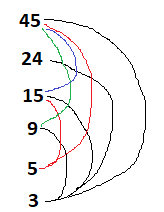
\includegraphics{admhw3ex10a.png}
\end{figure}

\item List the maximal and minimal elements.

Maximal: \bk{45, 24}. \tab Minimal: \bk{3, 5}

\item Is there a greatest element? A least element?

There is no element greater than nor less than all others.

\item Find all upper bounds of \bk{3, 5}. Find the least upper bound of \bk{3, 5}, if it exists.

UB(\bk{3, 5}): \bk{15, 45}. \tab LUB(\bk{3, 5}): \bk{15}

\item Find all the lower bounds of \bk{15, 45}. Find the greatest lower bound of \bk{15, 45}, if it exists.

LB(\bk{15, 45}): \bk{3, 5, 15}. \tab GLB(\bk{15, 45}): \bk{15}

\elist

}

\ssc{Exercise 11}{

Prove the following:

\balist
\item There is exactly one greatest element of a poset, if such an element exists.

Suppose \exs a, b \mem a poset P, such that a and b are the greatest elements of P.

Then a \gre x and b \gre x \fa x \mem P.

So a \gre b and b \gre a.

Thus, a \eql b.

\item There is exactly one maximal element in a poset with a greatest element.

Let P be a poset and let a be the greatest element in P.

Let b \mem P such that b $\neq$ a.

Then, by definition, a \lse b.

Thus, a is the only maximal element in P.

\item The least upper bound of a set in a poset is unique if it exists.

Let P be a poset and a \mem P.

Suppose \exs \uw{U}{1} and \uw{U}{2} \mem P such that \uw{U}{1} and \uw{U}{2} are least upper bounds for a and \uw{U}{1} $\neq$ \uw{U}{2}

Then, by definition, \uw{U}{1} \lse \uw{U}{2} and \uw{U}{2} \lse \uw{U}{1}.

Hence, \uw{U}{1} \eql \uw{U}{2}
\elist

}

\ssc{Exercise 12}{

Determine whether these posets are lattices.

\balist
\item (\bk{1, 3, 6, 9, 12}; $\vert$)

No, 9 join 6 doesn't have a LUB.

\item (\bk{1, 5, 25, 125}; $\vert$)

Yes.

\item (\bz; \gre)

Yes, but it's not a complete lattice.

\item ($\mathcal{P}$(S), \sbs), where $\mathcal{P}$(S) is the power set of a set S.

Yes.

\elist

}

\ssc{Exercise 13}{

Show that every totally ordered set is a lattice.

Let T be a totally ordered set, and let a, b \mem T.

Since T is totally ordered, either a \lse b or b \lse a.

Case:
\bilist
\item a \lse b

Then a meet b \eql a, and a join b \eql b.

\item b \lse a

Then b meet a \eql b, and b join a \eql a.

\elist

Hence, any two elements have a LUB and GLB.

}

\ssc{Exercise 14}{

Show that every finite lattice has a least element and a greatest element.

\

Let L be a finite lattice.

Suppose there are two least elements in L: \uw{l}{1}, \uw{l}{2} such that \uw{l}{1} $\neq$ \uw{l}{2}

Let l \eql \uw{l}{1} meet \uw{l}{2} (which exists because L is a lattice)

Case:

\bilist
\item l \eql \uw{l}{1}: a contradiction, since \uw{l}{2} is the least element.
\item l \eql \uw{l}{2}: a contradiction, since \uw{l}{1} is the least element.
\item l $\neq$ \uw{l}{1} and l $\neq$ \uw{l}{2}: a contradiction, since \uw{l}{1} and \uw{l}{2} are the least elements.
\elist

Thus, the least element in L is unique, if it exists.

Let A \eql \uw{a}{1} meet \uw{a}{2} meet ... \uw{a}{n} where n \eql \av{L} and \uw{a}{i} \mem L

Since A exists and is the least possible element, L has a least element.

WLOG, the same is true for a greatest element. (can I do this?)



}

\ssc{Exercise 15}{

Give an example of an infinite lattice with 

\balist
\item neither a least nor a greatest element.

(\bz, \lse)

\item a least but not a greatest element.

(\uf{\bz}{+}, \lse)

\item a greatest but not a least element.

(\uf{\bz}{-}, \lse)

\item both a least and a greatest element.

(\uf{\bq}{[0, 1]}, \lse)

\elist

}

\ssc{Exercise 16}{

Show that in any lattice (x \lgnd y) \lgnd z \eql x \lgnd (y \lgnd z). Note: (x \lgnd y) \lgnd z \lse x \lgnd (y \lgnd z) was shown in class.)

\

Proof of (x \lgnd y) \lgnd z \lse x \lgnd (y \lgnd z):

Z \lse Z

(X \lgnd Y) \lgnd Z \lse Z \bpth{1}

We also know:

(X \lgnd Y) \lgnd Z \lse X \lgnd Y \lse X \bpth{2}

(X \lgnd Y) \lgnd Z \lse X \lgnd Y \lse Y \bpth{3}

And:

(X \lgnd Y) \lgnd Z \lse X \lgnd Z by \bpth{1} and \bpth{2}

And:

(X \lgnd Y) \lgnd Z \lse X \lgnd (Y \lgnd Z) by \bpth{1}, \bpth{2} and \bpth{3}

\newpage

Proof of (x \lgnd y) \lgnd z \gre x \lgnd (y \lgnd z):

X \gre X

X \gre X \lgnd (Y \lgnd Z)

\

Y \lgnd Z \gre X \lgnd (Y \lgnd Z)

\

Y \gre Y \lgnd Z \gre X \lgnd (Y \lgnd Z)

Z \gre Y \lgnd Z \gre X \lgnd (Y \lgnd Z)

Thus,

(X \lgnd Y) \lgnd Z \gre X \lgnd (Y \lgnd Z)



}

\ssc{Exercise 17}{

Show that in any lattice x \lgor (x \lgnd y) \eql x. Note: the dual absorption law was shown in class.

\

X \lgor (X \lgnd Y) \gre X \bpth{1}

\

X \lgnd Y \lse X

X \lgor (X \lgnd Y) \lse X \lgor X \eql X

X \lgor (X \lgnd Y) \lse X \bpth{2}

By \bpth{1}, \bpth{2}, and antisymmetry, 

X \lgor (X \lgnd Y) \eql X



}

\ssc{Exercise 18}{

Show that any lattice x \lgor (y \lgnd z) \lse (x \lgor y) \lgnd (x \lgor z). Note: the dual distributive inequality was shown in class.

\

X \lgor Y \gre X

X \lgor Y \gre Y \gre Y \lgnd Z

X \lgor Y \gre X \lgor (Y \lgnd Z)

X \lgor Z \gre X \lgor (Y \lgnd Z) 

(X \lgor Y) \lgnd (X \lgor Z) \gre X \lgor (Y \lgnd Z)

}

\ssc{Exercise 19}{

Show that the two distributive equalities are equivalent. That is, x \lgor (y \lgnd z) \eql (x \lgor y) \lgnd (x \lgor z) if, and only if, x \lgnd (y \lgor z) \eql (x \lgnd y) \lgor (x \lgnd z).

\lra

WTS: x \lgor (y \lgnd z) \eql (x \lgor y) \lgnd (x \lgor z) \rar x \lgnd (y \lgor z) \eql (x \lgnd y) \lgor (x \lgnd z).

x \lgor (y \lgnd z) \eql (x \lgor y) \lgnd (x \lgor z)

(x \lgnd y) \lgor (x \lgnd z) \eql (x \lgor y) \lgnd (x \lgor z)

(x \lgnd y) \lgor (x \lgnd z) \eql x \lgnd (y \lgor z)

\lla 

WTS: x \lgnd (y \lgor z) \eql (x \lgnd y) \lgor (x \lgnd z) \rar x \lgor (y \lgnd z) \eql (x \lgor y) \lgnd (x \lgor z)

(x \lgnd y) \lgor (x \lgnd z) \eql x \lgnd (y \lgor z)

(x \lgnd y) \lgor (x \lgnd z) \eql (x \lgor y) \lgnd (x \lgor z)

x \lgor (y \lgnd z) \eql (x \lgor y) \lgnd (x \lgor z)

}

\ssc{Exercise 20}{

Show that the distributive law implies the modular law. That is, if a lattice satisfies one (hence both, from problem 19), then (x \lse z \rar x \lgor (y \lgnd z) \eql (x \lgor y) \lgnd z).

\

WTS:

x \lgor (y \lgnd z) \eql (x \lgor y) \lgnd (x \lgor z) or x \lgnd (y \lgor z) \eql (x \lgnd y) \lgor (x \lgnd z) \rar (x \lse z \rar x \lgor (y \lgnd z) \eql (x \lgor y) \lgnd z)

\

x \lse x \lgor y and x \lse z \rar x \lse (x \lgor y) \lgnd z

y \lgnd z \lse y \lse x \lgor y and y \lgnd z \lse z \rar y \lgnd z \lse (x \lgor y) \lgnd z

x \lgor (y \lgnd z) \lse (x \lgor y) \lgnd z

\

x \gre x \lgnd y and x \lse z \rar x \gre (x \lgnd y) \lgor z

y \lgor z \gre y \gre x \lgnd y and y \lgor z \gre z \rar y \lgor z \gre (x \lgnd y) \lgor z

x \lgor (y \lgnd z) \gre (x \lgor y) \lgnd z

\

Hence,

x \lgor (y \lgnd z) \eql (x \lgor y) \lgnd z

}

\ssc{Exercise 21}{

Check if the lattice \uw{N}{5} is distributive.

\ 

I checked. It isn't. Just kidding, here's why:

Let's look at Z \lgnd (Y \lgor X) \eql (Z \lgnd Y) \lgor (Z \lgnd X)

\

Z \lgnd (Y \lgor X)

Z \lgnd 1

Z

\

And:

\

(Z \lgnd Y) \lgor (Z \lgnd X)

0 \lgor X

X

\

This is saying Z \eql X, which is not true.

}
\end{document}